\documentclass[a4paper, 12pt]{article} % report for longer pieces

% Packages
\usepackage[utf8]{inputenc}
\usepackage{geometry}
\usepackage{setspace}
\usepackage{helvet} % Load Arial-like font
\usepackage{graphicx} % for inserting graphs & images
\usepackage{tocloft} % Package to customize the ToC
\usepackage{tocbibind} % Automatically adds the lists to the ToC
\usepackage{ragged2e} % Provides the \justifying command
\usepackage{indentfirst} % first line indented IF justified is on
\usepackage{parskip}
\usepackage{sectsty}
\usepackage{etoolbox} % Include etoolbox for conditional comparison

\usepackage{tabularx} % Tables respecting the margins
\usepackage{booktabs}
\usepackage{caption}
\usepackage{longtable}
\usepackage{float}

\usepackage{tikz}    % generating visualization w/o data

\usepackage{apacite} % For APA citation
\usepackage{natbib}  % For handling bibliographies

\usepackage{hyperref}
\hypersetup{
  colorlinks = true, % Ensures links are colored, not boxed
  linkcolor = black, % Color for internal links like sections
  citecolor = blue,  % Ensures citation links are blue
  urlcolor = blue,  % Color for URL links
  filecolor = black, % Color for file links
  menucolor = black, % Color for Acrobat menu links
  anchorcolor = black, % Color for anchor text
  linktoc = all % links everything in TOC, LOF, and LOT
}

\usepackage{doi} % doi as hyperlink
\renewcommand{\doitext}{} % avoid double doi in refs

%\usepackage{appendix}
\usepackage[titletoc]{appendix}
\newcommand{\listappendixname}{Appendix Directory}
\newlistof{appendixitems}{appdir}{\listappendixname}
\renewcommand{\cftappdirtitlefont}{\bfseries\fontsize{13pt}{15}\selectfont}

\usepackage{amsmath} %equations



%%%%%%%%%%%%%%%%%%%% DOCUMENT FORMATTING %%%%%%%%%%%%%%%%%%%%

% Setting the margins
\geometry{
  top = 2.5cm,
  bottom = 2.5cm,
  left = 2.5cm, %inner
  right = 1.5cm %outer
}

% Section headers in 13pt
\sectionfont{\fontsize{13pt}{15}\selectfont}

% Subsection headers in 12pt
\subsectionfont{\fontsize{12pt}{14}\selectfont}

% Subsubsection headers in 12pt
\subsubsectionfont{\fontsize{12pt}{14}\selectfont}

% No space between paragraphs
\setlength{\parskip}{0\baselineskip} %same {0pt plus 1pt}

% Set line spacing
\setstretch{1.5} % Change the line spacing to 1.5

% Changing font sizes for ToC, LoF, and LoT
\renewcommand{\cfttoctitlefont}{\normalfont\bfseries\fontsize{13pt}{15}\selectfont}
\renewcommand{\cftloftitlefont}{\normalfont\bfseries\fontsize{13pt}{15}\selectfont}
\renewcommand{\cftlottitlefont}{\normalfont\bfseries\fontsize{13pt}{15}\selectfont}

% Customize space between section number and title
\makeatletter
\renewcommand\@seccntformat[1]{%
  \ifstrequal{#1}{section}{%
    \csname the#1\endcsname\hspace{1.4em} % Adjust space for sections only
  }{%
    \ifstrequal{#1}{subsection}{%
      \csname the#1\endcsname\hspace{0.3em} % Adjust space for subsubsections
    }{%
      \csname the#1\endcsname\hspace{-0.5em} % Default spacing for others
    }
  }
}

\makeatother


%%%%%%%%%%%%%%%%%%%%%%%%%% Document %%%%%%%%%%%%%%%%%%%%%%%%%

\begin{document}

% Cover page
\begin{titlepage}
\vspace*{-2cm} % Adjust the value to reduce the top margin as needed
\singlespacing

    
    \begin{flushright}
    \includegraphics[width = 7cm]{images/JGU-logo_schriftzug.jpg} % Adjust width as needed
    \end{flushright}
    \vspace{2cm}
    
    \begin{flushleft}
    \large
    Johannes-Gutenberg University Mainz \\
    Faculty of Law and Economics \\
    Chair or Institute:  \\
    Advisor: Name of your advisor\\
    \end{flushleft}
    \vspace{2cm} % Adjusted spacing for title block
    
       \centering
    Topic:\\
    \LARGE
    \textbf{Main Title: \\
    \Large
    Secondary title} \\
    \vspace{1cm}
    \large
    Master's thesis for obtaining the academic degree: \\
    Add your degree and name of your programm \\
    \vspace{2cm} % Adjusted spacing for right block
    
    \begin{flushleft}
    \large
    \begin{tabular}{@{}l@{\hspace{0.5cm}}l} % Adding horizontal space between label and detail
        Submitted by: & \textbf{Your Name} \\[0.25cm] % Vertical spacing added here
        Student ID: & 00000000 \\[0.25cm]
        Address: & Address, \\[0.25cm]
        & PLZ \\[0.25cm]
        Telf.: & 00000000000 \\[0.25cm]
        Email: & uni email \\[0.25cm]
        & private email
    \end{tabular}
    \vspace{2cm}
    
    \large
    Place, date
    \end{flushleft}

\end{titlepage}


% Start Roman numeral page numbering
\pagenumbering{Roman}

% No page number on the first page
\thispagestyle{empty}


% Acknowledgements & Dedication
\centering
\section*{Acknowledgments} % ACKNOWLEDGMENTS
\begin{flushleft}
\justifying
\textit{First and foremost, I thank ...}
\end{flushleft}
\vspace{0.5cm}

\begin{flushleft}
\justifying
\textit{I would also like to place on record my sincere thanks to ...}
\end{flushleft}
\vspace{0.5cm}

\begin{flushleft}
\justifying
\textit{A special thanks to ...}
\end{flushleft}
\vspace{1cm}


\section*{Dedication} % DEDICATION
\begin{flushleft}
\justifying
\textit{To my ...}
\end{flushleft}
\vspace{0.5cm}

\newpage


% Set the page counter to 3
\setcounter{page}{3}

% Abstract %
\centering
\section*{Abstract}
\justifying
\noindent
Lorem ipsum dolor sit amet, consectetur adipiscing elit. Nam lacinia ultrices felis, et scelerisque velit bibendum vel. In hac habitasse platea dictumst. Praesent sit amet leo et erat vulputate consequat non vitae risus. Curabitur varius, turpis ut varius vestibulum, nisi mi sollicitudin turpis, id ultricies velit lorem a est. Vestibulum auctor consequat libero, a euismod libero fringilla nec. Ut vel varius urna, vitae egestas ligula. Morbi ac nulla eu metus tincidunt suscipit. Curabitur sed lacus et orci interdum consequat et ut eros. Phasellus luctus leo at libero vestibulum, sed volutpat lectus dictum.

\vspace{0.5cm} % Add some vertical space before the signature line
\begin{flushleft}
    \noindent\rule{\textwidth}{0.4pt} % Create a horizontal line across the page
\vspace{0.5cm}
\textbf{Keywords:} word1, word2, etc. \\
\vspace{2cm}
\end{flushleft}
\newpage

% Table of contents
%\pagebreak
\centering
\renewcommand{\contentsname}{Table of Contents} % name of the ToC
\renewcommand{\cftsecleader}{\cftdotfill{\cftdotsep}} % style .....
\addtocontents{toc}{\protect\setcounter{tocdepth}{-1}}
\tableofcontents
\addtocontents{toc}{\protect\setcounter{tocdepth}{2}} % or whatever depth you want
\newpage

% Lists of Figures and Tables
\listoffigures
\vspace{2cm}

\listoftables
\newpage


% Appendix Directory
%\section*{Appendix Directory}
\phantomsection
\addcontentsline{toc}{section}{Appendix Directory}
\setlength{\cftbeforesecskip}{0pt} 
\listofappendixitems  % This prints the custom Appendix Directory
\newpage


% Abbreviations
\section*{Abbreviations}
\addcontentsline{toc}{section}{Abbreviations}
\begin{tabularx}{\textwidth}{@{}lX@{}}
    FTP & File Transfer Protocol \\
    http & Hypertext Transfer Protocol \\
    https & Hypertext Transfer Protocol Secure \\
    WWW & World Wide Web \\
\end{tabularx}
\vspace{2cm}
\newpage


% Switch to Arabic numeral page numbering
\clearpage
\pagenumbering{arabic}
\raggedright % all left-sided
% Set line spacing
\setstretch{1.5}

% All sections
\onehalfspacing
\section{Introduction}\label{sec:intro}
\vspace{-0.5cm}

\justifying
Start your intro here

Citing multiple authors' works like this \citep[see][]{Brüderl2024, Huinink2011, Kreyenfeld2013} or a single one \citep[refer to][]{Schneider2021}.
However, citing the author in the text appears as follows: \cite{Bozoyan2021}. Furthermore, to cite a specific page, you will need: \citep[see][p. XX]{Goldin2024}.

Add as many paragraphs as you need.

Referring to different sections in texts: This thesis comprises eight sections, commencing with this introduction, and is structured as follows. 
\textbf{\hyperref[sec:literature]{Section 2}} provides a literature review based on ... . Moreover, \textbf{\hyperref[sec:empiricaldata]{Section 3}}
delves in ... . A descriptive analysis is performed in \textbf{\hyperref[sec:descriptive]{Section 4}}, aiming to identify trends and relationships in
the data before conducting the subsequent econometric methods described in \textbf{\hyperref[sec:methodology]{Section 5}}. Furthermore,
\textbf{\hyperref[sec:results]{Section 6}} proceeds to interpret the results from the base models, whereas \textbf{\hyperref[sec:furthernanalysis]{Section 7}}
provides further analysis, such as the mechanisms and extra robustness checks. Finally, this thesis concludes with \textbf{\hyperref[sec:discussion]{Section 8}},
which further discusses the limitations and sets the stage for future research on the topic.




% End of the Intro

\onehalfspacing
\section{Literature Review}\label{sec:literature}
\vspace{-0.5cm}
\justifying
Start your literature review here. Note the guidance on correctly citing in the introduction.

\subsection{Subtopic1}\label{sec:litrev1}
\vspace{-0.3cm}
\justifying
Remember, in the case of subsections, always at least two are needed. Otherwise, you do not need them and may proceed to the next section.

\subsection{Subtopic2}\label{sec:litrev2}
\vspace{-0.3cm}
\justifying
Continue...


\subsection{Subtopic3}\label{sec:litrev3}
\vspace{-0.3cm}
\justifying
Continue...




% End of this section

\onehalfspacing
\section{Empirical Data}\label{sec:empiricaldata}
\vspace{-0.5cm}

\subsection{Name of your Dataset}\label{sec:namedata}
\vspace{-0.3cm}
\justifying
E.g., this thesis analyses the XX waves of the YY dataset... 


\subsection{DF's Inconveniences}\label{sec:inconvenience}
\vspace{-0.3cm}
\justifying
As noted in the introduction, this subsection describes any inconveniences encountered during the data preparation ... .


\subsection{Dependent Variables}\label{sec:dependent}
\vspace{-0.3cm}
\justifying
Describe your dependent vars in a paragraph format:
\textit{Dep Var 1}: I use ... .

\textit{Dep Var 2}: More so ... .

\textit{Dep Var 3}: Continue ... .


\subsection{Independent Variables}\label{sec:independent}
\vspace{-0.3cm}
\justifying
In my thesis, having ... .

Starting a table looks, e.g., so:

\setlength{\tabcolsep}{5pt}
\begin{table}[htbp]
\centering
\captionsetup{justification = raggedright, singlelinecheck = false, skip = 2pt}
\caption{\textbf{Sample Size}}\label{tab:sample_size}
\begin{tabular}{lccccccccc} % Extend the number of columns to accommodate side-by-side panels
\toprule
                    & \multicolumn{4}{c}{Panel A} 
                    & \multicolumn{4}{c}{Panel B} \\
                    \cmidrule(lr){2-5} \cmidrule(lr){6-9} &
                    \multicolumn{2}{c}{Females} & \multicolumn{2}{c}{Males} & \multicolumn{2}{c}{Females} & \multicolumn{2}{c}{Males} \\
                    \cmidrule(lr){2-3} \cmidrule(lr){4-5} \cmidrule(lr){6-7} \cmidrule(lr){8-9}
                    & N & \% & N & \% & N & \% & N & \% \\
\midrule
\textbf{Category1:} \\
Dep Var 1 &2,444 &47.64 &2,218 &43.16  &4.899 &49.06 &4.042 &40.48\\
\textbf{Category2:} \\
Dep Var 2 &2,544 &49.50 &2,337 &45.48 &5,232 &52.40 &4,305 &43.11\\
\textbf{Category3:}\\
Dep Var 3 &2,651 &51.59 &2,470 &48.06 &5,448 &54.56 &4,529 &45.36\\
\midrule
Observations &2,653 &51.75 &2,474 &48.25 &5,451 &54.59 &4,534 &45.41\\
\bottomrule
\end{tabular}
\parbox{\textwidth}{\raggedright
\vspace{0.5em}
\textbf{Source}: ADD YOUR SOURCE.
\newline\textbf{Notes}: Add Notes if needed. e.g., your p-value significant starts explained. \\
}
\end{table}

This is how an element from the appendix can be referenced (see \textbf{\hyperref[tab:appendix-A1]{Appendix A1}}).

\subsection{Final Samples}\label{sec:finalsample}
\vspace{-0.3cm}
\justifying
Your data after all the cleaning, manipulation, and transformation is done.


%End of this Section.

\onehalfspacing
\section{Descriptive Analysis}\label{sec:descriptive}
\vspace{-0.5cm}
Start here with some descriptive analysis.

\subsection{Subtopic1}\label{sec:desc1}
\vspace{-0.3cm}
\justifying
Adding some figures \textbf{\hyperref[fig:DEPPP]{Figure 1}}.

\begin{figure}[H]    % important for where you need the elements located
    \centering
    \captionsetup{justification = raggedright, singlelinecheck = false}
    \includegraphics[width = \columnwidth]{images/DEGdpPPP.png}
    \caption{\textbf{Name of the figure}}
    \label{fig:DEPPP}
\end{figure}


\subsection{Subtopic2}\label{sec:desc2}
\vspace{-0.3cm}
\justifying
Continue...


\subsection{Subtopic3}\label{sec:desc3}
\vspace{-0.3cm}
\justifying
Continue...



% End of the section.

\onehalfspacing
\section{Empirical Methodology}\label{sec:methodology}
\vspace{-0.3cm}
As briefly discussed in \textbf{\hyperref[sec:dependent]{Subsection 3.3}}, this thesis employs ... :

introducing TikZ:

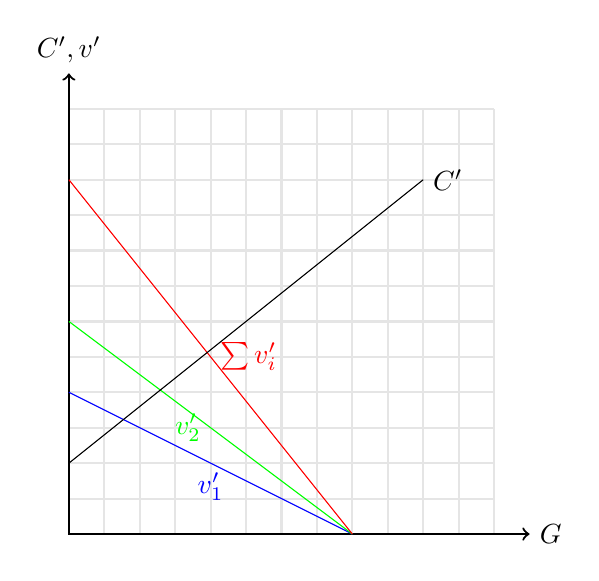
\begin{tikzpicture}[scale = 0.9]
		\draw[thick, step = 0.5cm, color = gray!20] (0,0) grid (6,6);
		\draw[thick, step = 0.5cm, color = gray!20, opacity = 0.3] (0,0) grid (6,6);
		\draw [<->,thick] (0,6.5) node (yaxis) [above] {$C' , v'$}
		|- (6.5,0) node (xaxis) [right] {$G$};
		\draw[blue] (0,2) -- node[below]{$v^{\prime}_1$} (4,0) ;
		\draw[green] (0,3) -- node[below, left]{$v^{\prime}_2$} (4,0);
		\draw[red]  (0,5) -- node[above, right]{$\sum v^{\prime}_i$}(4,0) ;
		\draw[black] (0,1) -- (5,5) node[right]{$C'$};
	\end{tikzpicture}


\subsection{Model 1}\label{sec:model1}
\vspace{-0.3cm}
\justifying
In the first empirical model, I define $Y_{it}$ as the dependent variable for individual $i$ at time $t$. For this model, the dependent variables are the \textit{Dep Var 1}, ... :

\vspace{-0.3cm}
\begin{equation}
Y_{it} = \alpha_i + \beta_1\text{DepVar1}_{it} + \beta'X'_{it} + \epsilon_{it}
\tag{1}
\end{equation}

\noindent
Moreover, the model incorporates the vector $X'_{it}$, which includes control variables to improve the precision of the estimates ... 


\subsection{Model 2}\label{sec:model2}
\vspace{-0.3cm}
\justifying
Analog to above...




% End of this section.

\onehalfspacing
\section{Base Results}\label{sec:results}
\vspace{-0.5cm}
In this section, I focus on the effects of ... .

\subsection{Category 1}\label{sec:cat1}
\vspace{-0.3cm}
\justifying
\textit{Dep Var 1}: In examining the impact of ... .


\subsection{Category 2}\label{sec:cat2}
\vspace{-0.3cm}
\justifying
\textit{Dep Var 2}: When exploring the ... .



\subsection{Category 3}\label{sec:cat3}
\vspace{-0.3cm}
\justifying
\textit{Dep Var 3}: The last outcome of interest is ... .





% This section ends here

\onehalfspacing
\section{Further Analysis}\label{sec:furthernanalysis}
\vspace{-0.5cm}

\subsection{Mechanisms}\label{sec:heterogeneity}
\vspace{-0.3cm}
\justifying
As reviewed, the heterogeneity of ... .

\subsubsection{Mechanism 1}\label{sec:mech1}
\vspace{-0.3cm}
\justifying
\textit{Dep Var 1/2/3}: After ... .


\subsubsection{Mechanism 2}\label{sec:mech2}
\vspace{-0.3cm}
\justifying
\textit{Dep Var 1/2/3}: The coefficients for ... .


\subsection{Further Robustness Checks}\label{sec:robustextra}
\vspace{-0.3cm}
\justifying
Text starts here

\subsubsection{Robustness 1}\label{sec:rob1}
\vspace{-0.3cm}
\justifying
\textit{Dep Var 1/2/3}: With the addition of ... .


\subsubsection{Robustness 2}\label{sec:rob2}
\vspace{-0.3cm}
\justifying
\textit{Dep Var 1/2/3}: There are some remarkable differences after ... .



% End of this section

\onehalfspacing
\section{Discussion}\label{sec:discussion}
\vspace{-0.5cm}
\justifying
This thesis aimed to explore the research gaps regarding ... .






% Finalizing
\clearpage
\pagenumbering{Roman}
% Set specific page number
\setcounter{page}{9} % Example: start from Roman numeral VIII

% Appendices
\centering
\appendix
\addcontentsline{toc}{section}{Appendices} % Adds "Appendices" to the main Table of Contents

% Resetting counters for tables and figures to ensure separate numbering in the appendix
\setcounter{table}{1}
\setcounter{figure}{1}

% Prefix table and figure numbers with 'A' to denote Appendix
\renewcommand{\thetable}{A\arabic{table}}
\renewcommand{\thefigure}{A\arabic{figure}}

% Redefine the caption command (within) the appendix to not add entries to LoT or LoF

\makeatletter
\let\oldcaption\caption
\renewcommand{\caption}[1]{
    \def\@tempa{figure}
    \def\@tempb{table}
    \ifx\@captype\@tempa % Check if it's a figure
        \oldcaption*{\figurename\ \thefigure: #1}
        \addcontentsline{appdir}{subsection}{\figurename\ \thefigure\hspace{1em}#1}
    \else\ifx\@captype\@tempb % Check if it's a table
        \oldcaption*{\tablename\ \thetable: #1}
        \addcontentsline{appdir}{subsection}{\tablename\ \thetable\hspace{1em}#1}
    \fi
    \fi
}
\makeatother

% Commands to add appendix entries; to call these manually if automatic captioning isn't suitable
\newcommand{\addappendixentry}[1]{
    \addcontentsline{appdir}{subsection}{\thetable\hspace{1em}#1}
}


\begin{appendices}

% Appendix A1 Descriptive Stats
\setlength{\tabcolsep}{3pt}
\renewcommand{\arraystretch}{0.8} % Adjust the factor
\begin{table}[H]
\setcounter{table}{1}
\centering
\captionsetup{justification = raggedright, singlelinecheck = false, skip = 2pt}
\caption{\textbf{Descriptive Statistics}}
\label{tab:appendix-A1}
\begin{tabular}{lcccc}
\toprule
 & \multicolumn{2}{c}{Females} & \multicolumn{2}{c}{Males} \\
\cmidrule(lr){2-3} \cmidrule(lr){4-5}
 & Mean & SD & Mean & SD \\
\midrule
\textbf{Main Outcomes of Interest:} \\
Dep Var 1 & 7.80 & (0.62) & 7.82 & (0.69) \\
Dep Var 2 & 6.88 & (0.75) & 7.44 & (0.75) \\
Dep Var 3 & 73.66 & (44.06) & 83.77 & (36.88) \\
\textbf{Background Characteristics:} \\
Var1 & 24.27 & (42.88) & 44.30 & (49.68) \\
Var2 & 45.42 & (49.80) & 41.55 & (49.29) \\
Var3 (\%) & 24.20 & (42.84) & 34.36 & (47.50) \\
Var4 & 12.46 & (3.34) & 12.65 & (3.21) \\
\midrule
Observations & 2,653 &  & 2,474 &  \\
\bottomrule
\end{tabular}
\parbox{\textwidth}{\raggedright
\vspace{0.5em}
%\textbf{Notes}: \\
\textbf{Source}: Add your source.
}
\end{table}
\newpage















\end{appendices}


% Use of AI
\centering
\section*{Use of AI Tools}
\addcontentsline{toc}{section}{Use of AI Tools} % Adds "Use of AI" to the main Table of Contents
\raggedright

List not only all the AI tools you use for the development of your thesis, but also a copy of the prompts and outputs you received from those engines!


% Bibliography
\centering
\bibliographystyle{apacite}
\bibliography{Bibliography}

% Declaration of Authorship
\centering
\include{Authorship}




\end{document}
